\documentclass[a4paper,kulak]{kulakarticle} %options: kul or kulak (default)

\usepackage[utf8]{inputenc}
\usepackage[dutch]{babel}
\usepackage{graphicx}
\usepackage{flafter}
\usepackage{pdfpages}

\date{Academiejaar 2020 -- 2021}
\address{
	Bachelor in de ingenieurswetenschappen \\
	Probleemoplossen en ontwerpen, deel 2 \\
	Benjamin Maveau, Kevin Truyaert}
\title{Overzicht ontwerpspecificaties}
\author{Team 1: Safety First}

\begin{document}


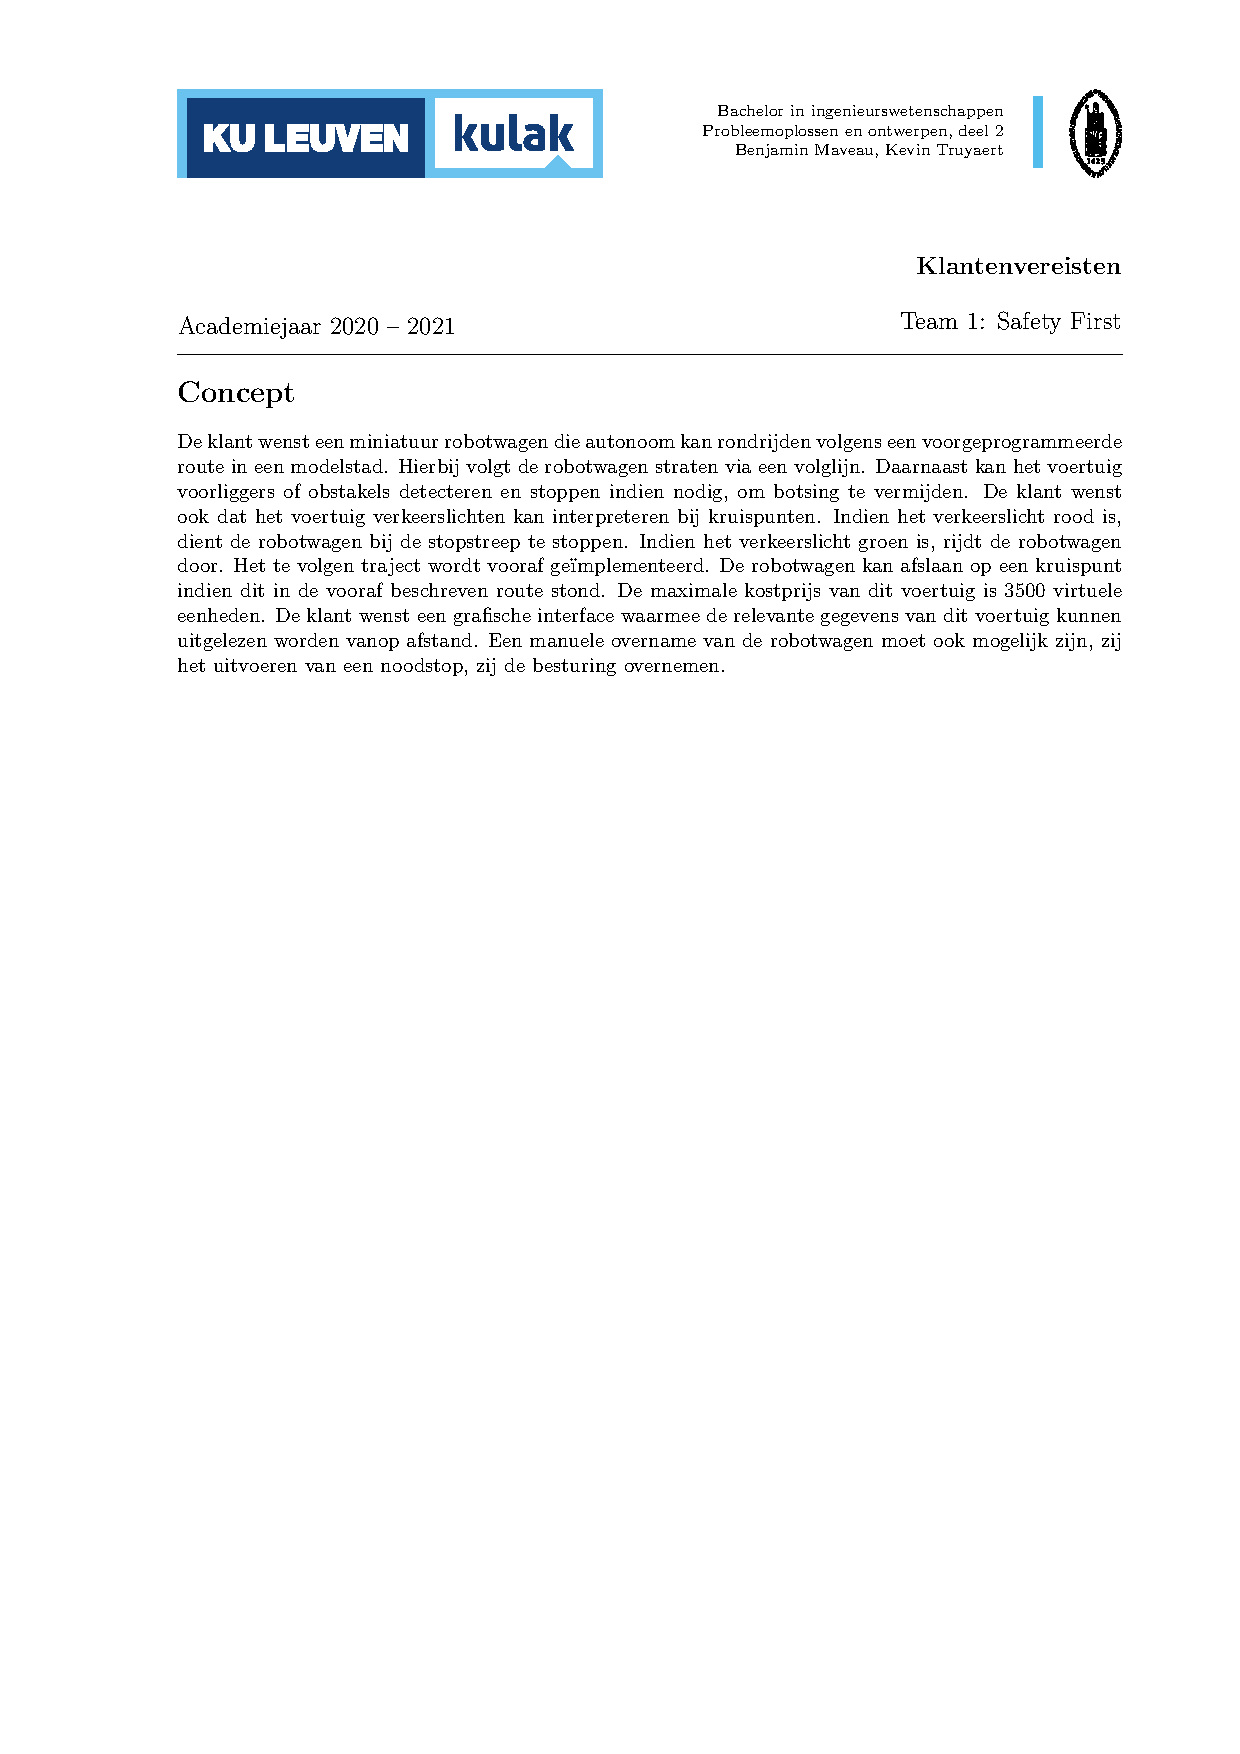
\includepdf{klantenvereisten}
	
\maketitle
	
\section*{Ontwerpspecificaties}
De klant wenst een zelfrijdend wagentje dat zich volgens een voorgeprogrammeerde route door een modelstad beweegt. De modelstad bestaat uit negen identieke kruispunten opgesteld in een vierkant die zich op een afstand van 1 meter van elkaar bevinden. Figuren \ref{kruispunt} en \ref{techtekkruispunt} tonen een voorbeeld van een van die kruispunten.
	
\begin{figure}[h]
	\centering
	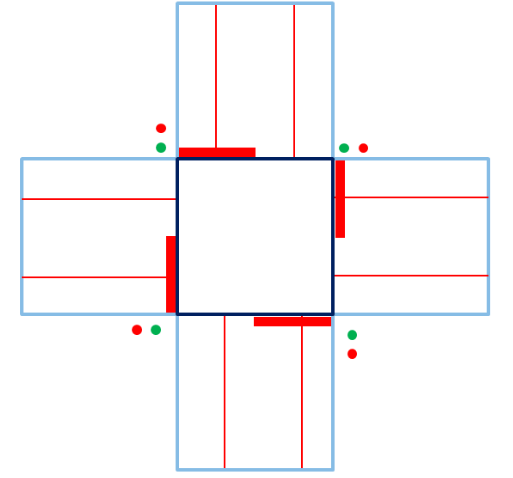
\includegraphics[width=0.45\textwidth]{kruispunt.png}
	\caption{Bovenaanzicht van een kruispunt (figuur ontleend aan \cite{teamopdracht})}
	\label{kruispunt}
\end{figure}
	
	
Het robotvoertuig volgt hierbij een lijn van 25mm dik aan de hand van een reflectiesensor, dit zijn de dunne rode lijnen op figuur \ref{kruispunt}. Deze volglijn is een donkere lijn op een heldere ondergrond of een heldere lijn op een donkere ondergrond. De lengte van een te volgen straat is 1 meter en de breedte ervan bedraagt 0.5 meter. Op deze baan bewegen voertuigen zich rechts in de heenrichting en links in de terugrichting. De maximale, totale breedte van het voertuig bedraagt dus 25 cm. Aan een kruispunt interpreteert het voertuig een rood-groen verkeerslicht. De verkeerslichten zijn gemonteerd op een tafelonderstel (zie figuur \ref{techtekkruispunt}). Aangezien de hoogte hiervan 300 mm is, is dit ook de maximale hoogte van het te bouwen voertuig. Het midden van het verkeerslicht bevindt zich op 7.5 cm boven de grond. Zoals te zien op de technische tekening \ref{verkeerslicht} is dit ook de plaats waar de kleurled zich in het verkeerslicht bevindt. Het verkeerslicht is gemonteerd aan de voorkant van de tafelpoot, zodat de wagen het verkeerslicht langs de rechterkant moet detecteren, zoals ook figuur \ref{kruispunt} suggereert.  Indien het verkeerslicht rood is, stopt het voertuig bij de stopstreep. Deze stopstreep is 50 mm dik en 25 cm lang, zoals we kunnen afleiden uit de rode dikke lijnen in figuur \ref{kruispunt}. Indien het verkeerslicht groen is, rijdt het wagentje door of slaat het af, naargelang de gevraagde voorgeprogrammeerde route.
	
\begin{figure}[h]
	\centering
	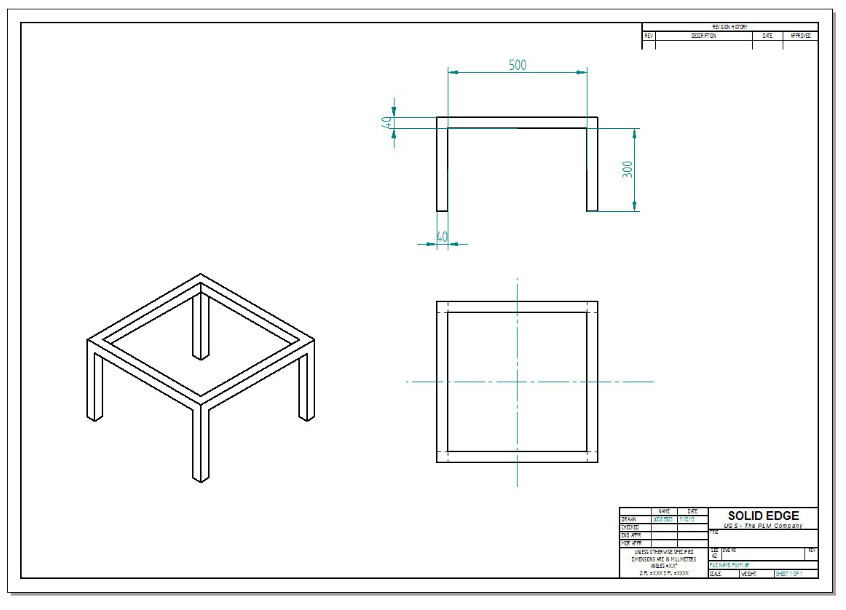
\includegraphics[width=0.65\textwidth]{tafelstel.png}
	\caption{Technische tekening van een kruispunt (figuur ontleend aan \cite{teamopdracht})}
	\label{techtekkruispunt}
\end{figure}
	
\begin{figure}
	\centering
	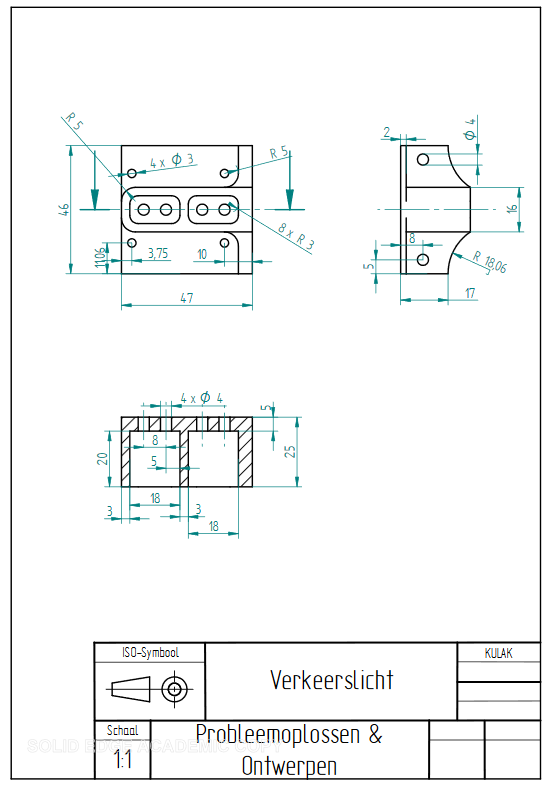
\includegraphics[width=0.6\textwidth]{verkeerslicht.png}
	\caption{Technische tekening van een verkeerslicht (figuur ontleend aan \cite{teamopdracht} )}
	\label{verkeerslicht}
\end{figure}
	
Het wagentje kan ook voorliggers detecteren via een afstandssensor. Indien het een voorligger detecteert, vertraagt het wagentje of stopt het om zo een botsing te vermijden.
Het te volgen traject wordt een week op voorhand bekend gemaakt en kan dan al geprogrammeerd worden.	De componenten van het prototype mogen verbonden worden via een breadboard. De definitieve versie van het voertuig moet wel via een printplaat kunnen functioneren. Voor de microcontroller dient gebruik te worden gemaakt van een NI myRIO of Raspberry Pi. Tussen de microcontroller en de motoren dient een motorshield te worden aangebracht, gezien dit een terugloopbeveiliging bevat die beschadiging van de microcontroller voorkomt. Het voertuig haalt zijn energie uit een batterij. De maximale kostprijs van het prototype bedraagt 3500 virtuele eenheden.
	
De klant wenst ook dat er een draadloze informatieoverdracht is tussen het voertuig en een computer op afstand. Deze draadloze informatieoverdracht verloopt via LabVIEW en er is ook een grafische interface beschikbaar. Via deze interface kan een noodstop worden uitgevoerd of de volledige besturing van het robotvoertuig overgenomen worden.
	
\bibliography{referenties_ontwerpspecificaties}
\bibliographystyle{unsrt}
	

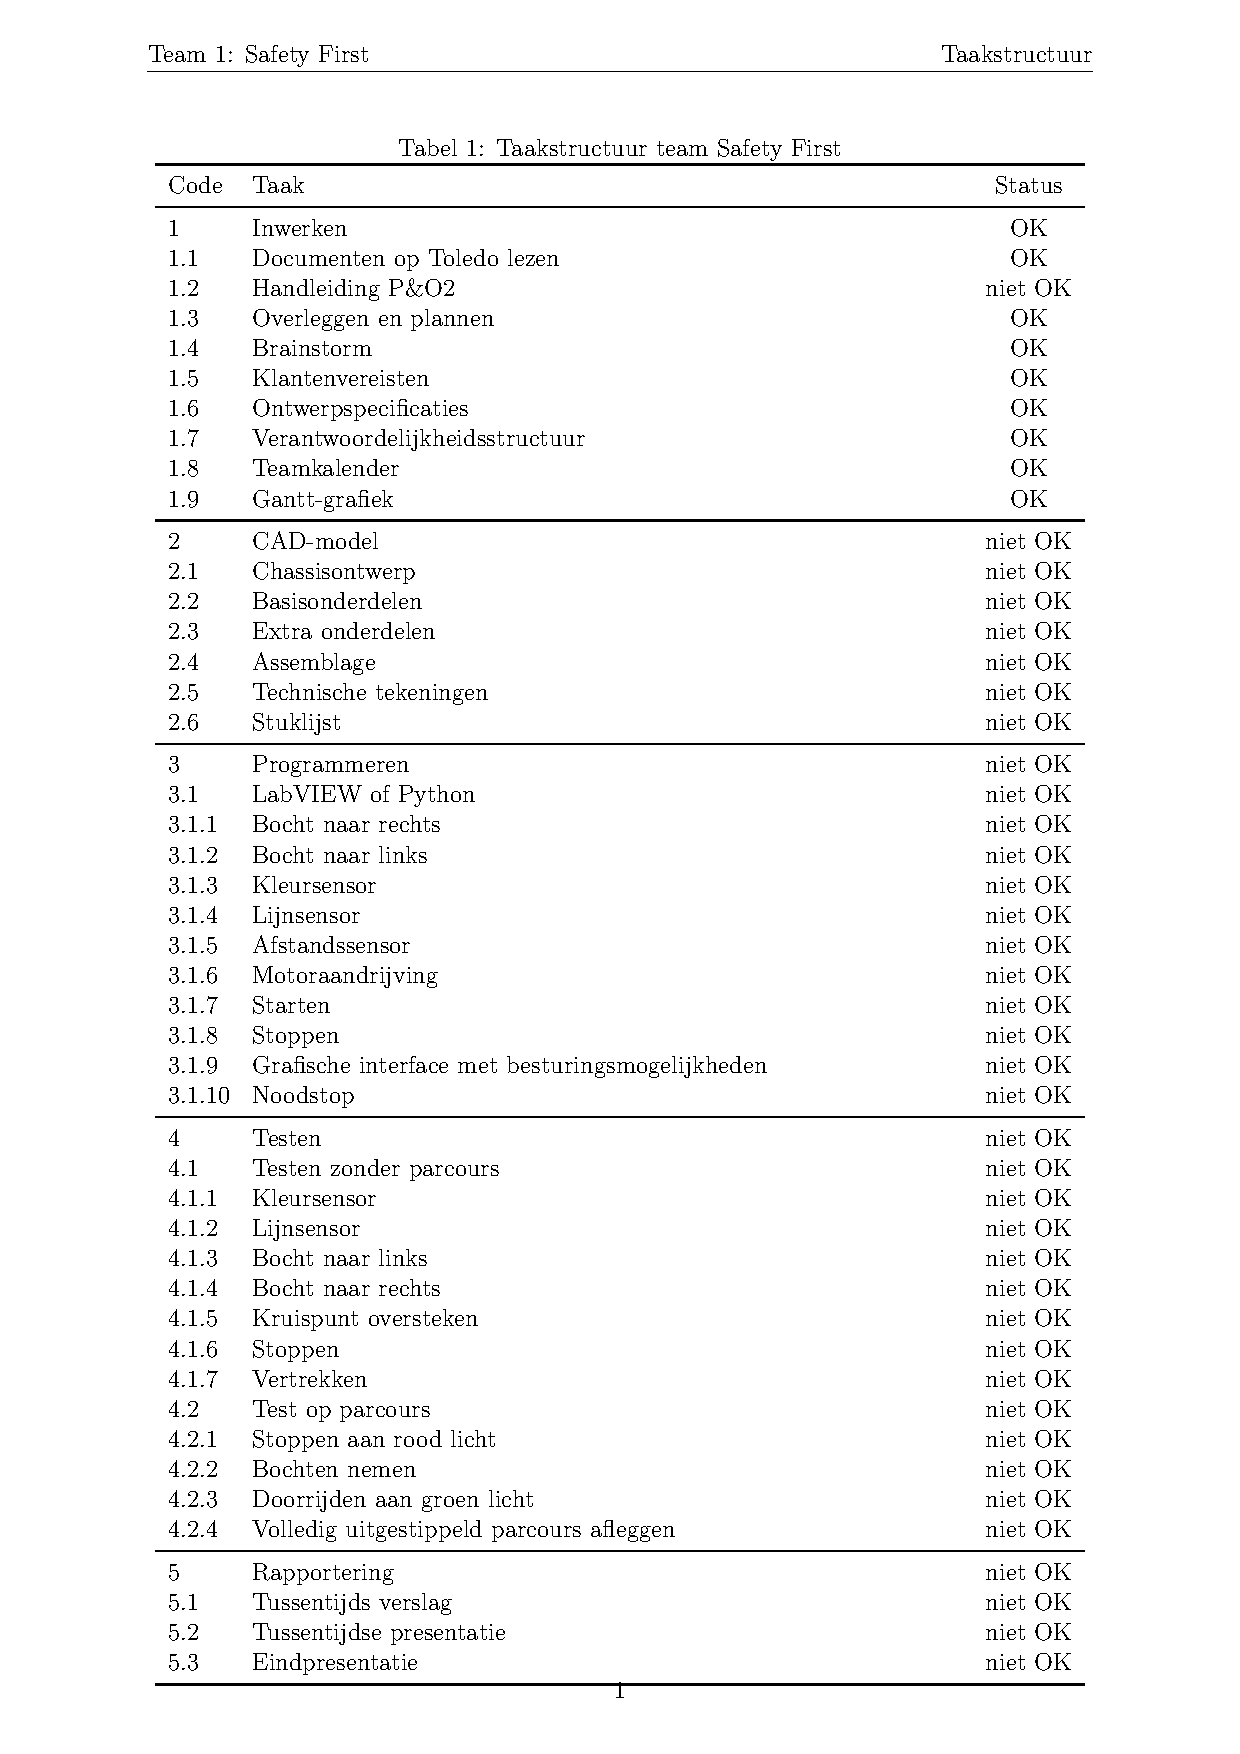
\includepdf[pages={1-}]{taakstructuur}
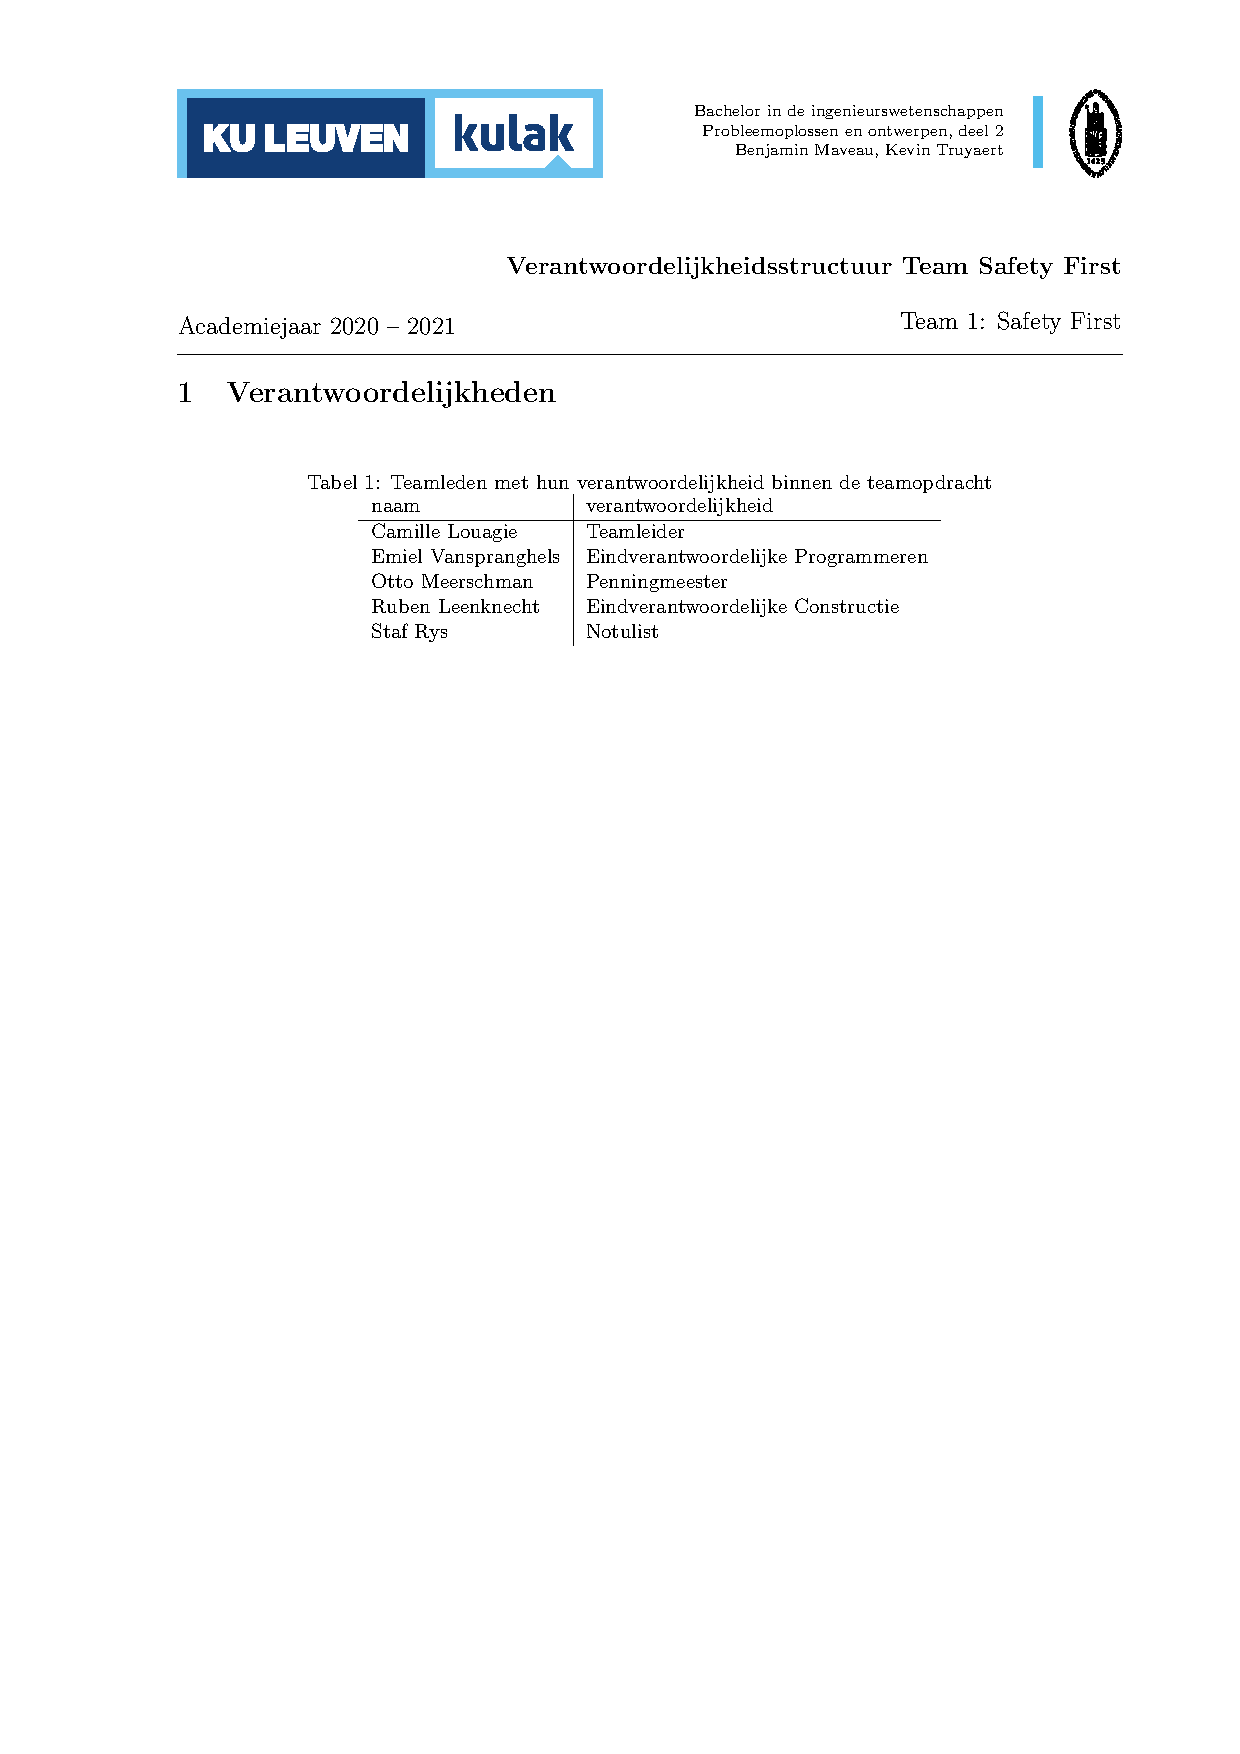
\includepdf{verantwoordelijkheidsstructuur}
%\includepdf{teamkalender}
\KOMAoptions{paper=landscape,pagesize}
\recalctypearea
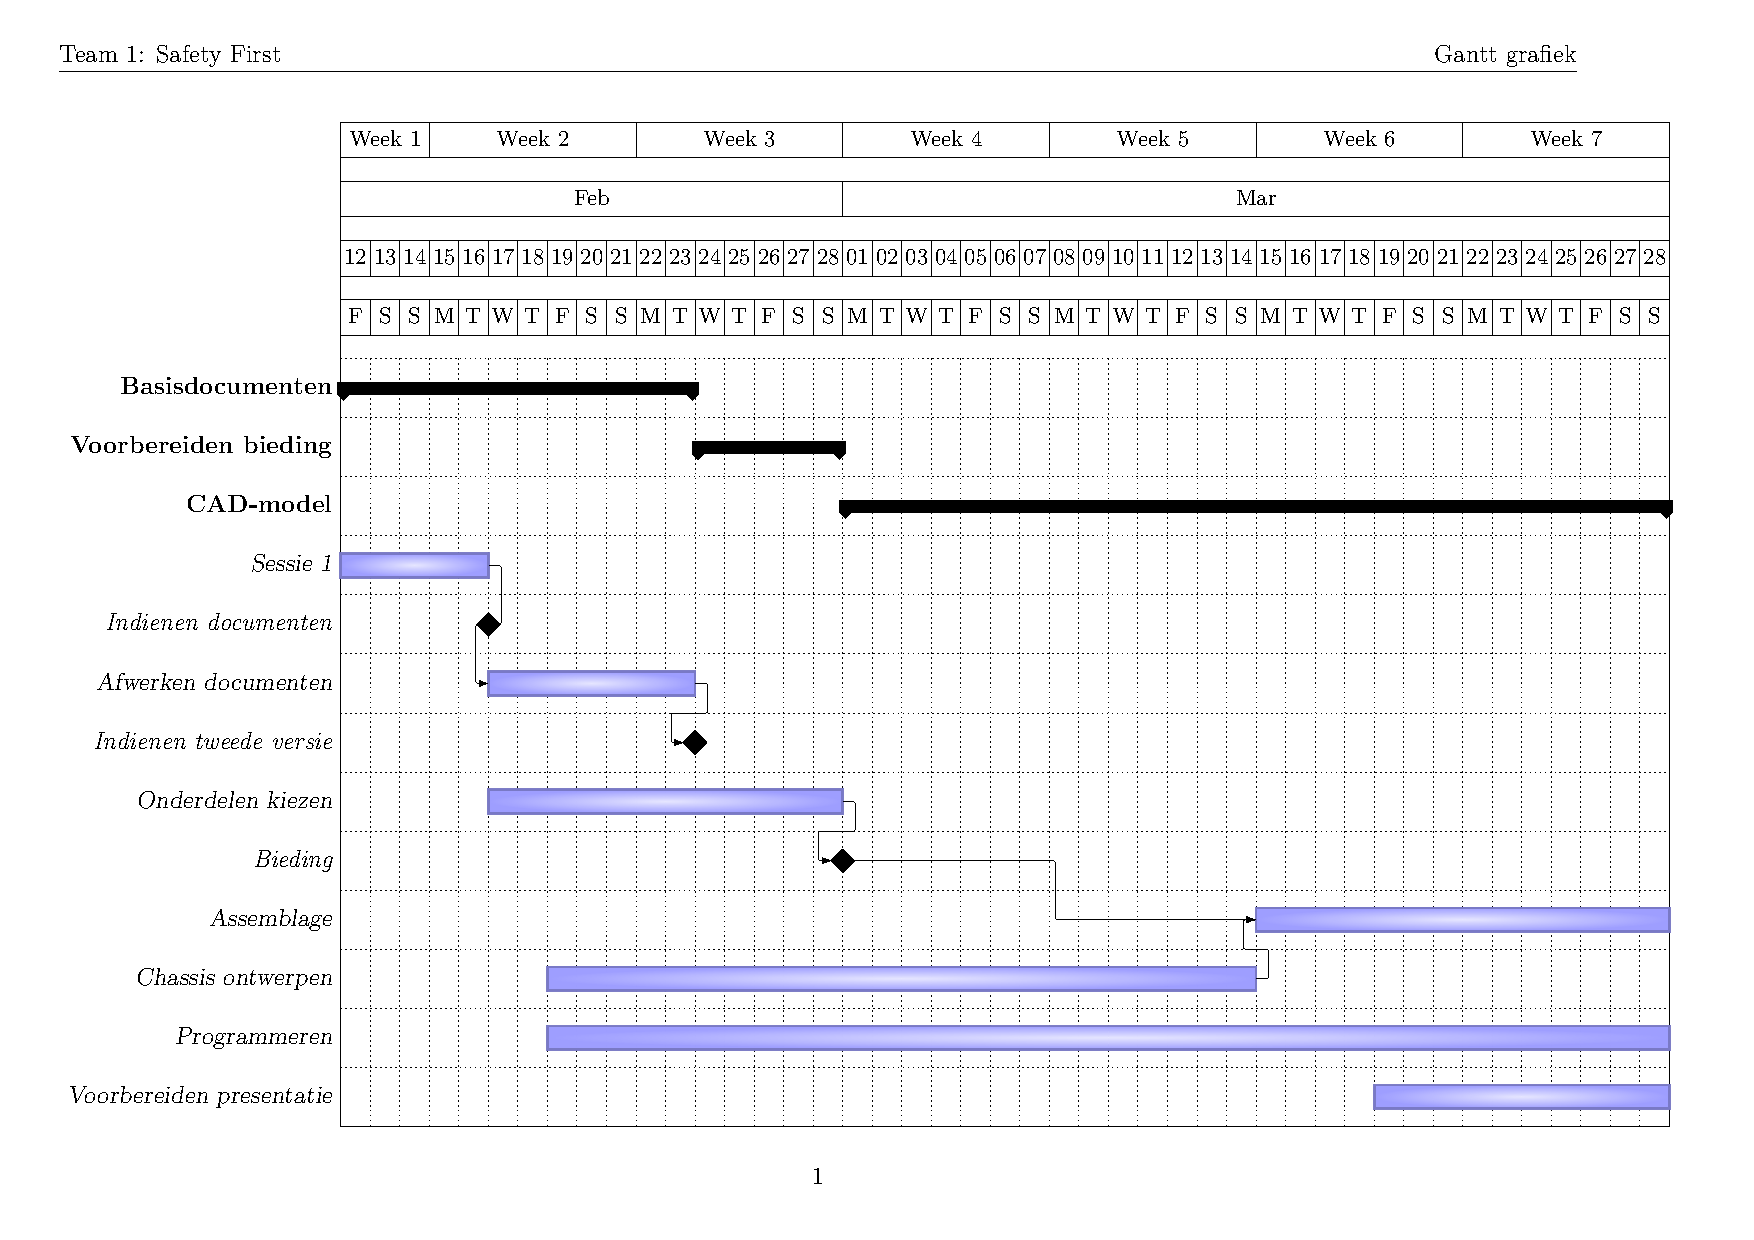
\includepdf[pages=1]{ganttchart}
\includepdf[pages=2]{ganttchart}

\end{document}